\documentclass[10pt]{article}

%\textwidth=7in
%\textheight=9.5in
%\topmargin=-1in
%\headheight=0in
%\headsep=.5in
%\hoffset=-1in

\usepackage[top=1in,left=1in,right=1in,bindingoffset=5mm,twoside]{geometry}

\usepackage{amssymb}
\usepackage{amsmath}
\usepackage{enumitem}
\usepackage{framed}
\usepackage[framed]{ntheorem}
\usepackage{dsfont}
\usepackage{bm}
\usepackage{quoting}
\usepackage{setspace}
\usepackage{xifthen}
\usepackage{textcomp}
\usepackage{nameref}
\usepackage{tikz}
\usepackage{graphicx}




\newcommand\onestar{$\star$}
\newcommand\twostar{$\star\star$}
\newcommand\threestar{$\star\star\star$}



\theoremstyle{margin}
\theorembodyfont{\normalfont}
\theoremseparator{.}
\theorempreskipamount=\baselineskip
\theorempostskipamount=-1.5em

\theoremprework{\begin{onehalfspace}} \theorempostwork{\end{onehalfspace}}
\newtheorem{defn}{Definition}  %[chapter]

\theoremprework{\begin{onehalfspace}} \theorempostwork{\end{onehalfspace}}
\newtheorem{example}[defn]{Example}

\theoremprework{\begin{onehalfspace}} \theorempostwork{\end{onehalfspace}}
\newtheorem{axiom}[defn]{Axiom}

\newtheorem{corol}[defn]{Corollary}

\newtheorem{conjecture}[defn]{Conjecture}


\theoremprework{\begin{onehalfspace}} \theorempostwork{\end{onehalfspace}}
\newtheorem{thmex}[defn]{Example Theorem}

\theoremheaderfont{\scshape}
\theoremindent\parindent
\newtheorem*{proofex}[defn]{Example Proof}
\theoremheaderfont{\normalfont\bfseries}
\theoremindent0cm

\theoremstyle{plain}
\theorembodyfont{\normalfont}
%\theoremindent=\parindent
%\theoremseparator{.}

\theorempreskipamount=-2em
\theorempostskipamount=-.75em

\newframedtheorem{thm}[defn]{Theorem}

\newframedtheorem{thm1}[defn]{\raisebox{.1em}{\onestar} Theorem}
\newframedtheorem{thm2}[defn]{\raisebox{.1em}{\twostar} Theorem}
\newframedtheorem{thm3}[defn]{\raisebox{.1em}{\threestar} Theorem}


\newframedtheorem{lemma}[defn]{Lemma}
\newframedtheorem{lemma1}[defn]{\raisebox{.1em}{\onestar} Lemma}
\newframedtheorem{lemma2}[defn]{\raisebox{.1em}{\twostar} Lemma}
\newframedtheorem{lemma3}[defn]{\raisebox{.1em}{\threestar} Lemma}

\newcommand\stmtword{Proposition}
\newframedtheorem{stmt}[defn]{\stmtword}

\newframedtheorem{stmt1}[defn]{\raisebox{.1em}{\onestar} \stmtword}
\newframedtheorem{stmt2}[defn]{\raisebox{.1em}{\twostar} \stmtword}
\newframedtheorem{stmt3}[defn]{\raisebox{.1em}{\threestar} \stmtword}


\newframedtheorem{exer}[defn]{Exercise}

\newframedtheorem{exer1}[defn]{\raisebox{.1em}{\onestar} Exercise}

\newframedtheorem{exer2}[defn]{\raisebox{.1em}{\twostar} Exercise}

\newframedtheorem{exer3}[defn]{\raisebox{.1em}{\threestar} Exercise}


\newframedtheorem{progexer}[defn]{Programming Exercise}


\newenvironment{exersoln}[1]{\textbf{Exercise #1 Solution.}\begin{quote}}{\end{quote}}
\newenvironment{stmtsoln}[1]{\textbf{\stmtword\ #1 Proof.}\begin{quote}}{\end{quote}}
\newenvironment{thmsoln}[1]{\textbf{Theorem #1 Proof.}\begin{quote}}{\end{quote}}
\newcommand\answer{\par\textbf{\emph{Answer}.\ }}
\newcommand\proof{\par\textbf{\emph{Proof}.\ }}

\newenvironment{exenumerate}{\begin{enumerate}[label=(\alph*),leftmargin=3em]}{\end{enumerate}}
%\newenvironment{discussion}{\begin{quoting}[vskip=0pt]}{\end{quoting}}
\newenvironment{discussion}{\begin{leftbar}\noindent}{\end{leftbar}}
%\newenvironment{discussion}{}{}

\newcommand\defterm[1]{\emph{\textbf{#1}}}  % a term being defined
\newcommand\hint{\\ \emph{Hint:}\ }
\newcommand*{\happymac}{\hfill
\includegraphics[height=2em]{happymac.png}\\}

\newcommand\emptystring\epsilon
\newcommand\definedas{\ \equiv\ }
%\newcommand\implies\to
\newcommand*{\qed}{\hfill\ensuremath{\square}}

\newcommand\naturals{\mathds{N}}

\newcommand\setbuildsepname{colon}
\newcommand\setbuildsep{:}
\newcommand\setdef[1]{\left\lbrace #1 \right\rbrace}
\newcommand\setbuild[2]{\left\lbrace #1\ \setbuildsep\ #2 \right\rbrace}
\newcommand\union\cup
\newcommand\intersection\cap
\newcommand\setunion[2]{#1\,\union\,#2}
\newcommand\setintersection[2]{#1\,\intersection\,#2}
\newcommand\setconcat[2]{#1\,\circ\,#2}
\newcommand\setcomplement[1]{\overline{#1}}
\newcommand\setstar[1]{#1^{*}}
\newcommand\powerset[1]{\mathcal{P}(#1)}
\newcommand\setproduct[2]{#1 \times #2}
\newcommand\yields{\ \Rightarrow\ }
\newcommand\derives{\ \Rightarrow^*\ }

\newcommand\langof[1]{\mathcal{L}(#1)}

\newcommand\stringrev[1]{#1^{\mathcal{R}}}


\title{Written Work - Regular Languages: DFAs} 	% TITLE OF THESE EXERCISES/PROOFS
\author{Nadeem Abdul Hamid}      			% YOUR NAME HERE
\date{\today}							% CHANGE IF YOU WANT

\begin{document}

\maketitle

%%% NOTE: 
%%% The site http://madebyevan.com/fsm/ allows you to graphically draw finite state automata and then export them as LaTeX or various graphics formats.


\begin{exersoln}{73} % 73 is the number of the exercise
\begin{center}
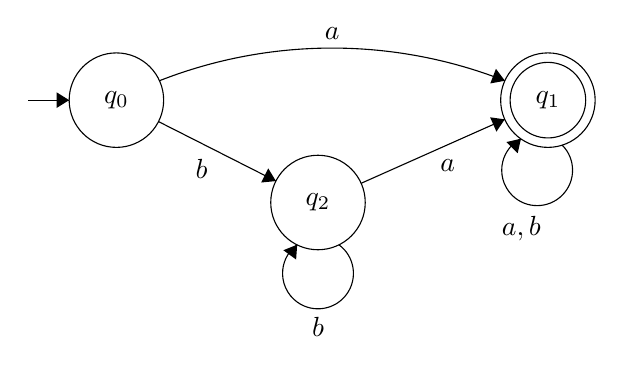
\begin{tikzpicture}[scale=0.2]
\tikzstyle{every node}+=[inner sep=0pt]
\draw [black] (6,-7.8) circle (3);
\draw (6,-7.8) node {$q_0$};
\draw [black] (33.4,-7.8) circle (3);
\draw (33.4,-7.8) node {$q_1$};
\draw [black] (33.4,-7.8) circle (2.4);
\draw [black] (18.8,-14.3) circle (3);
\draw (18.8,-14.3) node {$q_2$};
\draw [black] (8.733,-6.567) arc (111.42324:68.57676:30.025);
\fill [black] (30.67,-6.57) -- (30.1,-5.81) -- (29.74,-6.74);
\draw (19.7,-3.99) node [above] {$a$};
\draw [black] (34.3,-10.65) arc (45.25384:-242.74616:2.25);
\draw (31.71,-15.13) node [below] {$a,b$};
\fill [black] (31.69,-10.25) -- (30.77,-10.46) -- (31.48,-11.17);
\draw [black] (8.67,-9.16) -- (16.13,-12.94);
\fill [black] (16.13,-12.94) -- (15.64,-12.13) -- (15.19,-13.03);
\draw (11.41,-11.55) node [below] {$b$};
\draw [black] (20.123,-16.98) arc (54:-234:2.25);
\draw (18.8,-21.55) node [below] {$b$};
\fill [black] (17.48,-16.98) -- (16.6,-17.33) -- (17.41,-17.92);
\draw [black] (21.54,-13.08) -- (30.66,-9.02);
\fill [black] (30.66,-9.02) -- (29.73,-8.89) -- (30.13,-9.8);
\draw (27.03,-11.56) node [below] {$a$};
\draw [black] (0.4,-7.8) -- (3,-7.8);
\fill [black] (3,-7.8) -- (2.2,-7.3) -- (2.2,-8.3);
\end{tikzpicture}
\end{center}

Write out a 5-tuple giving a formal definition for the DFA\footnote{Designed using \texttt{http://madebyevan.com/fsm/}.} above.

	\answer    % precede your answers with \answer, proofs with \proof
	Give your answer here.
	\qed		% for coolness
\end{exersoln}

\begin{exersoln}{76}
Describe the language recognized by the DFA of Example~72.
\end{exersoln}

\begin{exersoln}{77}
Consider the DFA, $M = (\setdef{q_1, q_2}, \setdef{\textrm{0, 1}}, \delta, q_1, \setdef{q_2})$ with transition function $\delta$ given by
\[\begin{array}{c|cc}
 & \textrm{0} & \textrm{1} \\ \hline
 q_1 & q_1 & q_2 \\
 q_2 & q_1 & q_2
\end{array}\]

Draw a state diagram corresponding to the given DFA and describe in a single, concise English sentence the language that it recognizes.
\end{exersoln}

\begin{stmtsoln}{79}
All of the following languages over the alphabet $\Sigma_{\ref{stmt:dfas}} = \setdef{\texttt{a}, \texttt{b}}$ are regular.
\begin{itemize}
\item $L_1 = \setbuild{w}{\textrm{every \texttt{a} is immediately followed by a \texttt{b}}}$
\item $L_2 = \setbuild{w}{w~\textrm{contains an even number of \texttt{a}'s and an odd number of \texttt{b}'s}}$
\item $L_3 = \setbuild{w}{w~\textrm{contains the substring \texttt{baa}}}$
\item $L_4 = \setbuild{w}{w~\textrm{does not contain the substring \texttt{aab}}}$
\item $L_5 = \setbuild{w}{w~\textrm{has length at least 3 and its third symbol is a}~\texttt{b}}$
\item $L_6 = \setbuild{w}{w~\textrm{starts with \texttt{a} and has odd length, or starts with \texttt{b} and has even length}}$
\item $L_7 = \setbuild{w}{\textrm{every odd position of}~w~\textrm{is an}~\texttt{a}}$
\item $L_8 = \setdef{\emptystring, \texttt{a}}$
\item $L_9 = \emptyset$
\item $L_{10} = $ the set of all strings over $\Sigma_{\ref{stmt:dfas}}$ except the empty string
\end{itemize}
\end{stmtsoln}

\begin{exersoln}{80. Vowels in alphabetical order}
Let \[L_\alpha = \setbuild{w \in \setstar{\setdef{\texttt{a} - \texttt{z}}}}{\textrm{all five vowels}\ \texttt{a}, \texttt{e},
			\texttt{i}, \texttt{o}, \texttt{u}, \textrm{occur in alphabetical order in}~w}\]
So $L_\alpha$ contains words like \texttt{abstemious} and \texttt{facetious} but not \texttt{tenacious} or \texttt{tame}. Show that $L_\alpha$ is a regular language.
\end{exersoln}

\begin{exersoln}{81. Floating point numbers}
~\\Let 
\[L_{\mathrm{float}} = \setbuild{w}{w~\textrm{is the string representation of a floating point number}}\]
Assume the following syntax for floating point numbers:
\begin{itemize}
\item A floating point number is an optional sign, followed by a decimal number, followed by an optional exponent.
\item A decimal number may be of the form $x$ or $x.y$, where $x$ and $y$ are nonempty strings of decimal digits.
\item An exponent beings with \texttt{E} and is followed by an optional sign and then an integer.
\item An integer is a nonempty string of decimal digits.
\end{itemize}
The following strings are examples of floating point numbers:
\[\mathrm{+3.0, 3.0, 0.3E1, 0.3E+1, -0.3E+1, -3E8, 7}\]
Show that $L_{\mathrm{float}}$ is regular.
\end{exersoln}




%\begin{exersoln}{#}
%	
%	\answer
%	Give your answer here.
%\end{exersoln}



\end{document}